\chapter{Parity Vectors and the Syracuse Map}\label{chap:parity}

The rule ``halve if even, triple and add one if odd'' has two ingredients, a
multiplicative one and a parity test, and everything interesting about the
problem comes from the way they interact. This chapter isolates the parity
test. We record the sequence of parities along an orbit as a binary word, the
\emph{parity vector\index{parity vector}}, and show that over a block of $k$ steps the parity
vector and the residue of the starting value modulo $2^k$ determine each other
completely. This theorem of Terras\index{Terras, R.} and Everett\index{Everett, C. J.} is the single most useful fact about the
problem. It explains why the iteration looks random: a uniformly random
residue modulo $2^k$ produces a parity vector of $k$ independent fair coin
flips, exactly and not approximately. It gives the exact Geometric law of the
halving exponent $\vt(3n+1)$, the exact drift\index{drift} $\log(3/4)$ of the Syracuse
map, and, after passing to the $2$ adic integers, a conjugacy of the Collatz
map with the binary shift. And it yields the first genuine theorem about the
conjecture, that almost every positive integer eventually falls below itself.

All of these results are statements about ensembles of starting values. None
of them says anything about a particular orbit, and the reader should keep in
mind throughout the chapter where exactly that limitation enters.

\section{Three maps}\label{sec:ch2:maps}

\Cref{chap:intro} introduced three versions of the iteration. We now fix
them formally.

\begin{definition}[The three Collatz maps]\label{def:maps}
\leavevmode
\begin{enumerate}[label=(\roman*),leftmargin=2em]
\item The \emph{standard map} $T_0:\Z\to\Z$ is $T_0(n)=n/2$ for even $n$ and
  $T_0(n)=3n+1$ for odd $n$.
\item The \emph{accelerated map} $T:\Z\to\Z$ is $T(n)=n/2$ for even $n$ and
  $T(n)=(3n+1)/2$ for odd $n$.
\item The \emph{Syracuse map} $S$ is defined on odd integers by
  $S(n)=(3n+1)/2^{\vt(3n+1)}$, where $\vt(m)$ denotes the exponent of the
  largest power of $2$ dividing $m\neq0$. It maps odd integers to odd
  integers.
\end{enumerate}
We write $T_0^{(k)}$, $T^{(k)}$, $S^{(k)}$ for the $k$th iterates, with the
zeroth iterate the identity.
\end{definition}

The maps $T_0$ and $T$ are defined on all of $\Z$, the map $S$ on all odd
integers (since $3n+1\neq0$ for integer $n$), and all three send positive
integers to positive integers. The relations between them are
immediate from the definitions. For every integer $n$,
\begin{equation}\label{eq:ch2:TT0}
  T(n)=T_0^{(1+b)}(n),\qquad b=n\bmod2,
\end{equation}
because for odd $n$ the value $3n+1$ is even and $T$ simply performs the
forced halving at once. For odd $n$, with $k=\vt(3n+1)$,
\begin{equation}\label{eq:ch2:ST}
  S(n)=T^{(k)}(n)=T_0^{(k+1)}(n),
\end{equation}
since $T(n)=(3n+1)/2$ and the next $k-1$ values $(3n+1)/2^i$, $1\leq i<k$, are
even. Thus the orbit of $n$ under $T$ is obtained from its orbit under $T_0$
by deleting the even value that follows each odd value, and the orbit of an
odd $n$ under $S$ is the subsequence of odd values in either.

\begin{proposition}[Equivalence of the three maps]\label{prop:ch2:equiv}
Let $n\geq1$. The orbit of $n$ under $T_0$ contains $1$ if and only if its
orbit under $T$ contains $1$. If $n$ is odd, this happens if and only if its
orbit under $S$ contains $1$. If $n=2^a n'$ with $n'$ odd, the orbit of $n$
contains $1$ if and only if the orbit of $n'$ does.
\end{proposition}

\begin{proof}
The values deleted in passing from the $T_0$ orbit to the $T$ orbit are of the
form $3y+1$ with $y\geq1$ odd, hence at least $4$; so $1$ is never deleted, and
the two orbits contain $1$ together. For odd $n$, the $S$ orbit is the set of
odd values in the $T$ orbit, and $1$ is odd. Finally $T^{(a)}(2^a n')=n'$.
\end{proof}

Each map has its uses. The standard map\index{standard map} is the one in the statement of the
conjecture, and it has one structural property the others lack.

\begin{lemma}[No consecutive odd steps]\label{prop:nocons}
If $n$ is odd then $T_0(n)$ is even. Consequently the parity sequence
$b_j=T_0^{(j)}(n)\bmod2$ of any orbit of $T_0$ never contains two consecutive
ones.
\end{lemma}

\begin{proof}
If $n$ is odd then $3n$ is odd, so $3n+1$ is even.
\end{proof}

\Cref{prop:nocons} is trivial, but it is easy to transfer it by mistake to the
accelerated map\index{accelerated map}.

\begin{remark}[A pitfall: odd runs under the accelerated map]\label{rem:ch2:pitfall}
Under $T$ consecutive odd steps do occur. For odd $n$, $T(n)=(3n+1)/2$ is odd
exactly when $3n+1\equiv2\pmod4$, that is, when $n\equiv3\pmod4$. Thus
$T(3)=5$, $T(7)=11$, $T(11)=17$, and $T^{(2)}(7)=17>7$, an ascent over two
steps. A tempting but false argument runs: ``an odd step multiplies by about
$3/2$ and is followed by an even step dividing by $2$, so any two consecutive
steps of $T$ that begin with an odd one multiply by at most about $3/4$.'' The
first clause is true and the second is false, because under $T$ the halving
that follows the tripling has already been absorbed into the odd step. In fact
runs of odd steps under $T$ can be arbitrarily long: for $j\geq1$ and any odd
$a$, induction on $i$ gives
\[
  T^{(i)}(2^j a-1)=3^i2^{j-i}a-1,\qquad 0\leq i\leq j,
\]
so the orbit of $2^ja-1$ begins with $j$ consecutive odd steps and climbs to
$3^ja-1$. Any descent inequality over a fixed number of steps of $T$ must
accommodate these runs.
We return to this point in \cref{chap:lyapunov}: a Syracuse stride from an odd $x\geq3$, defined below, descends exactly when it contains at least two halvings (\cref{thm:stride}), and no fixed number of strides gives descent for every starting value (\cref{cor:ch4:multistride}).
\end{remark}

The Syracuse map\index{Syracuse map} compresses each passage from one odd value to the next, which we call a \emph{stride}, into a single step.
For odd $x$ write $k=\vt(3x+1)\geq1$. Then
\begin{equation}\label{eq:ch2:stride}
  \log S(x)-\log x=\log\Bigl(3+\frac1x\Bigr)-k\log2 .
\end{equation}
Since $2<3+1/x\leq4$ for $x\geq1$, the increment is positive when $k=1$ and
negative when $k\geq2$ (for $x=1$, $k=2$ and the increment is $0$). The whole
question of descent is therefore a question about how often the halving
exponent $k$ equals $1$, and about the sizes of the larger values.

\begin{example}[The orbit of $27$ under the three maps]\label{ex:ch2:27}
The orbit of $27$ reaches $1$ after $111$ steps of $T_0$, $70$ steps of $T$,
and $41$ steps of $S$. The $41$ halving exponents along the Syracuse orbit are
\[
\begin{gathered}
  1,2,1,1,1,1,2,2,1,2,1,1,2,1,1,1,2,3,1,1,2,\\
  1,2,1,1,1,1,1,3,1,1,1,4,2,2,4,3,1,1,5,4,
\end{gathered}
\]
with sum $70$ and mean $70/41\approx1.707$.
The mean is below $2$, the value predicted by the Geometric law of \cref{sec:ch2:geom}; the climb itself happens in the first $32$ strides, whose exponents have mean $44/32=1.375<\lt$ and which take the orbit to its largest odd value $3077$.
The overall mean is above $\lt\approx1.585$, which is forced, as we shall see in \cref{chap:divergence}, for any orbit that reaches $1$.
\end{example}

\section{Parity vectors and the Terras bijection}\label{sec:ch2:terras}

From now on, unless stated otherwise, we work with the accelerated map\index{accelerated map} $T$ on
$\Z$.

\begin{definition}[Parity vector]\label{def:ch2:parity}
For $n\in\Z$ and $k\geq1$, the \emph{parity vector\index{parity vector}} of length $k$ of $n$ is
\[
  v_k(n)=\bigl(n\bmod2,\ T(n)\bmod2,\ \ldots,\ T^{(k-1)}(n)\bmod2\bigr)\in\{0,1\}^k .
\]
We write $m_k(n)$ for the number of ones in $v_k(n)$, the number of odd steps
among the first $k$, and $m_0(n)=0$.
\end{definition}

For example $v_3(3)=(1,1,0)$, since $3\mapsto5\mapsto8$, and $v_4(5)=(1,0,0,0)$,
since $5\mapsto8\mapsto4\mapsto2$. The basic computation is the following
lemma, which says how the orbit of $x$ responds when $x$ is perturbed by a
multiple of a power of $2$.

\begin{lemma}[Perturbation by a power of two]\label{lem:ch2:perturb}
Let $x,a\in\Z$ and $j\geq0$. For $0\leq i\leq j$,
\[
  T^{(i)}(x+2^ja)=T^{(i)}(x)+3^{m_i(x)}\,2^{\,j-i}\,a .
\]
In particular, for $i<j$ the values $T^{(i)}(x+2^ja)$ and $T^{(i)}(x)$ have the
same parity, so $v_j(x+2^ja)=v_j(x)$.
\end{lemma}

\begin{proof}
Induction on $i$. For $i=0$ there is nothing to prove. Suppose the identity
holds for some $i<j$, and put $y=T^{(i)}(x)$ and $y'=T^{(i)}(x+2^ja)=
y+3^{m_i(x)}2^{j-i}a$. Since $j-i\geq1$, $y'\equiv y\pmod2$. If $y$ is even
then $T(y')=y/2+3^{m_i(x)}2^{j-i-1}a$ and $m_{i+1}(x)=m_i(x)$. If $y$ is odd
then
\[
  T(y')=\frac{3y+1}{2}+3^{m_i(x)+1}2^{j-i-1}a ,
\]
and $m_{i+1}(x)=m_i(x)+1$. In both cases the identity holds at $i+1$.
\end{proof}

\begin{theorem}[Terras~\cite{terras1976}, Everett~\cite{everett1977}]\label{thm:terras}
For every $k\geq1$, the parity vector $v_k(n)$ depends only on $n\bmod2^k$,
and the induced map
\[
  \Phi_k:\Z/2^k\Z\to\{0,1\}^k,\qquad n\bmod2^k\mapsto v_k(n),
\]
is a bijection.
\end{theorem}

\begin{proof}
That $v_k(n)$ depends only on $n\bmod2^k$ is the case $j=k$ of
\cref{lem:ch2:perturb}. For injectivity, suppose $0\leq x<x'<2^k$ and
$v_k(x)=v_k(x')$. Let $j=\vt(x'-x)$, so $0\leq j<k$ and $x'=x+2^ja$ with $a$
odd. By \cref{lem:ch2:perturb} with $i=j$,
\[
  T^{(j)}(x')-T^{(j)}(x)=3^{m_j(x)}a ,
\]
which is odd. Hence $T^{(j)}(x)$ and $T^{(j)}(x')$ have different parities,
and since $j\leq k-1$ the vectors $v_k(x)$ and $v_k(x')$ differ in position
$j$, a contradiction. An injective map between two sets with $2^k$ elements is
a bijection.
\end{proof}

The proof shows a little more, which we record because it is the form used in
\cref{sec:ch2:adic}: if $\vt(x'-x)=j$ then the parity vectors of $x$ and $x'$
agree in positions $0,\ldots,j-1$ and differ in position $j$.

\begin{example}[Small moduli]\label{ex:ch2:small}
For $k=3$ the bijection $\Phi_3$ is
\[
\begin{array}{c|cccccccc}
n\bmod8 & 0&1&2&3&4&5&6&7\\ \hline
v_3(n) & 000&101&010&110&001&100&011&111
\end{array}
\]
Every word of length $3$ appears exactly once. Note that $7$ has parity vector
$111$, three odd steps in a row, in line with \cref{rem:ch2:pitfall}.
\end{example}

\begin{corollary}[Exact randomness of the first $k$ parities]\label{cor:ch2:iid}
Let $n$ be uniformly distributed on $\{1,2,\ldots,2^kN\}$ for some $N\geq1$, or
on $\Z/2^k\Z$. Then the entries of $v_k(n)$ are independent Bernoulli random
variables with parameter $\tfrac12$. Consequently $m_k(n)$ has the binomial
law with parameters $k$ and $\tfrac12$.
\end{corollary}

\begin{proof}
In both cases $n\bmod2^k$ is uniform on $\Z/2^k\Z$, so by \cref{thm:terras}
$v_k(n)$ is uniform on $\{0,1\}^k$, which is the law of $k$ independent fair
bits.
\end{proof}

\Cref{cor:ch2:iid} is the precise sense in which the Collatz iteration is
random. It is exact, but it has a horizon: the first $k$ parities of $n$ are
random when $n$ is random modulo $2^k$, and no statement is made about step
$k+1$ and beyond unless $n$ is random modulo a higher power of $2$.
For $n$ random modulo $2^k$, each step uses up one bit of the residue, and after $k$ steps the randomness is exhausted.

\section{The affine form of an iterate}\label{sec:ch2:affine}

The second basic fact is that $k$ steps of $T$ act on $n$ as an affine map
whose coefficients depend only on the parity vector\index{parity vector}.

\begin{proposition}[Affine form]\label{prop:ch2:affine}
For $n\in\Z$ and $k\geq0$,
\begin{equation}\label{eq:ch2:affine}
  2^k\,T^{(k)}(n)=3^{m_k(n)}\,n+c_k(n),
\end{equation}
where $c_0(n)=0$ and
\begin{equation}\label{eq:ch2:crec}
  c_{k+1}(n)=\begin{cases}3\,c_k(n)+2^k, & T^{(k)}(n)\text{ odd},\\
  c_k(n), & T^{(k)}(n)\text{ even}.\end{cases}
\end{equation}
Explicitly, if the odd steps occur at positions $0\leq i_1<i_2<\cdots<i_m\leq
k-1$ of the parity vector, with $m=m_k(n)$, then
\begin{equation}\label{eq:ch2:cexplicit}
  c_k(n)=\sum_{j=1}^{m}3^{\,m-j}\,2^{\,i_j}.
\end{equation}
In particular $c_k(n)$ depends only on $v_k(n)$, it is a nonnegative integer,
and it is positive as soon as $m_k(n)>0$.
\end{proposition}

\begin{proof}
Induction on $k$; the case $k=0$ is trivial. Write $x=T^{(k)}(n)$ and
$m=m_k(n)$, and assume $2^kx=3^mn+c_k(n)$. If $x$ is even then
$2^{k+1}T(x)=2^kx$, so the identity holds at $k+1$ with $m_{k+1}=m$ and
$c_{k+1}=c_k$. If $x$ is odd then
\[
  2^{k+1}T(x)=2^k(3x+1)=3\cdot2^kx+2^k=3^{m+1}n+3c_k(n)+2^k,
\]
and $m_{k+1}=m+1$. Unwinding the recursion, the odd step at position $i_j$
contributes $2^{i_j}$, which is then multiplied by $3$ once for each of the
$m-j$ later odd steps; this is \eqref{eq:ch2:cexplicit}.
\end{proof}

The identity \eqref{eq:ch2:affine}, with the positivity of $c_k$, is simple
enough to be checked by machine, and we have done so: it is one of the
statements proved in the Lean\index{Lean} proof assistant, by exactly the induction above,
in the formalization described in \cref{chap:cycles}. There is a second,
multiplicative way to see the same quantity. Multiplying the ratios
$T(y)/y$ along the orbit, each even value contributes $1/2$ and each odd value
$y$ contributes $(3+1/y)/2$, so for $n\geq1$
\begin{equation}\label{eq:ch2:product}
  \frac{2^kT^{(k)}(n)}{3^{m}n}=\prod_{\substack{0\leq i<k\\ T^{(i)}(n)\text{ odd}}}
  \Bigl(1+\frac{1}{3T^{(i)}(n)}\Bigr),
\end{equation}
and hence $c_k(n)=3^mn\bigl(\prod(1+1/(3T^{(i)}(n)))-1\bigr)$, the product
running over the same odd values.
The additive ones of the iteration are thus a small multiplicative correction
when the odd values are large, and \eqref{eq:ch2:product} is the form we use
in \cref{chap:cycles}.

\begin{example}\label{ex:ch2:c27}
The orbit of $27$ reaches $1$ after $70$ steps of $T$, with $m_{70}(27)=41$.
Then \eqref{eq:ch2:affine} reads $2^{70}=3^{41}\cdot27+c_{70}(27)$, and indeed
the sum \eqref{eq:ch2:cexplicit} evaluates to
$c_{70}(27)=195\,820\,718\,533\,800\,070\,543=2^{70}-27\cdot3^{41}$, about
$0.166\cdot2^{70}$.
\end{example}

Two consequences of \cref{prop:ch2:affine} will be used repeatedly.

\begin{corollary}[Explicit inverse of the Terras map]\label{cor:ch2:inverse}
For $w\in\{0,1\}^k$ with $m$ ones at positions $i_1<\cdots<i_m$, the unique
residue $n\bmod2^k$ with $v_k(n)=w$ is
\[
  n\equiv-3^{-m}\,c(w)\equiv-\sum_{j=1}^{m}3^{-j}2^{i_j}\pmod{2^k},
\]
where $c(w)$ is the sum \eqref{eq:ch2:cexplicit} and $3^{-1}$ denotes the
inverse of $3$ modulo $2^k$.
\end{corollary}

\begin{proof}
Reduce \eqref{eq:ch2:affine} modulo $2^k$: $0\equiv3^mn+c(w)$, and $3$ is
invertible modulo $2^k$.
\end{proof}

For example, $w=(1,1,0)$ has $c(w)=3\cdot2^0+2^1=5$ and $m=2$; since
$9\equiv1\pmod8$ we get $n\equiv-5\equiv3\pmod8$, as in \cref{ex:ch2:small}.

\begin{corollary}[Cycles]\label{cor:ch2:cycle}
Suppose $n\geq1$ and $T^{(k)}(n)=n$ for some $k\geq1$, and let $m=m_k(n)$.
Then $m\geq1$, $3^m<2^k$, and
\begin{equation}\label{eq:ch2:cyclen}
  n=\frac{c_k(n)}{2^k-3^m}.
\end{equation}
\end{corollary}

\begin{proof}
A cycle of positive integers cannot consist of halvings alone, so $m\geq1$ and
$c_k(n)>0$. By \eqref{eq:ch2:affine}, $(2^k-3^m)n=c_k(n)>0$.
\end{proof}

For the trivial cycle, $n=1$, $k=2$, $w=(1,0)$ gives $c=1$ and
$2^2-3=1$. The same formula holds on $\Z$ without the sign conclusion: the
negative cycle $-5\mapsto-7\mapsto-10\mapsto-5$ of $T$ has $w=(1,1,0)$,
$c=5$ and $2^3-3^2=-1$, so $n=-5$. Formula \eqref{eq:ch2:cyclen} turns the
search for cycles with a given parity word into a divisibility test, and the
inequality $3^m<2^k$ is the starting point of \cref{chap:cycles}.

\section{The Geometric law of the halving exponent}\label{sec:ch2:geom}

We turn to the Syracuse map\index{Syracuse map} and the halving exponent $k=\vt(3n+1)$. Define
\[
  a_j=\frac{4^{\lceil j/2\rceil}-1}{3},\qquad j\geq1,
\]
so that $a_1=a_2=1$, $a_3=a_4=5$, $a_5=a_6=21$, $a_7=a_8=85$. Since
$3a_j+1=4^{\lceil j/2\rceil}$ is divisible by $2^j$, $a_j$ is the inverse of
$-3$ modulo $2^j$.

\begin{proposition}[Exact Geometric law]\label{prop:geom}
Let $n$ be odd and $j\geq1$. Then $\vt(3n+1)\geq j$ if and only if
$n\equiv a_j\pmod{2^j}$. Consequently, if $n$ is uniformly distributed on the
odd residues modulo $2^M$, then
\begin{align*}
  \Prob\bigl(\vt(3n+1)\geq j\bigr)&=2^{-(j-1)}, && 1\leq j\leq M,\\
  \Prob\bigl(\vt(3n+1)=j\bigr)&=2^{-j}, && 1\leq j\leq M-1.
\end{align*}
Thus $\vt(3n+1)$ has the Geometric$(\tfrac12)$ law on $\{1,2,\ldots\}$ up to
the truncation imposed by the modulus, with mean $2$ and variance $2$ in the
limit.
\end{proposition}

\begin{proof}
$\vt(3n+1)\geq j$ means $3n\equiv-1\pmod{2^j}$, and since $3$ is invertible
modulo $2^j$ this congruence has the unique solution $n\equiv a_j$; it is odd
because $a_j$ is odd. Among the $2^{M-1}$ odd residues modulo $2^M$, exactly
$2^{M-j}$ reduce to $a_j$ modulo $2^j$, giving probability
$2^{M-j}/2^{M-1}=2^{-(j-1)}$. Subtracting consecutive values gives the law of
$\{\vt(3n+1)=j\}$ for $j\leq M-1$. The Geometric$(\tfrac12)$ law on
$\{1,2,\ldots\}$ has mean $\sum_{j\geq1}2^{-(j-1)}=2$ and variance
$(1-\tfrac12)/(\tfrac12)^2=2$.
\end{proof}

\begin{table}[t]
\centering
\caption{Residue classes for the halving exponent $k=\vt(3n+1)$ of odd $n$.
The second column gives the class modulo $2^j$ on which $k\geq j$, the third the class modulo $2^{j+1}$ on which $k=j$ exactly, and the last its proportion among the odd residues.}
\label{tab:ch2:geom}
\begin{tabular}{@{}cccc@{}}
\toprule
$j$ & $k\geq j$ & $k=j$ & $\Prob(k=j)$\\
\midrule
$1$ & $n\equiv1\pmod2$ & $n\equiv3\pmod4$ & $1/2$\\
$2$ & $n\equiv1\pmod4$ & $n\equiv1\pmod8$ & $1/4$\\
$3$ & $n\equiv5\pmod8$ & $n\equiv13\pmod{16}$ & $1/8$\\
$4$ & $n\equiv5\pmod{16}$ & $n\equiv5\pmod{32}$ & $1/16$\\
$5$ & $n\equiv21\pmod{32}$ & $n\equiv53\pmod{64}$ & $1/32$\\
$6$ & $n\equiv21\pmod{64}$ & $n\equiv21\pmod{128}$ & $1/64$\\
$7$ & $n\equiv85\pmod{128}$ & $n\equiv213\pmod{256}$ & $1/128$\\
$8$ & $n\equiv85\pmod{256}$ & $n\equiv85\pmod{512}$ & $1/256$\\
\bottomrule
\end{tabular}
\end{table}

\Cref{tab:ch2:geom} lists the classes for small $j$. The law is classical: it
is the one stride case of \cref{cor:ch2:iid}. For odd $n$, $T(n)=(3n+1)/2$ and the halving
exponent equals one plus the number of zeros that follow the leading one of
the parity vector\index{parity vector} before the next one. Under the uniform law on parity vectors
that number of zeros is Geometric on $\{0,1,2,\ldots\}$ with parameter
$\tfrac12$.

Over the odd integers below $2^{20}$, the exponent $k=j$ occurs exactly
$2^{19-j}$ times for each $j\leq19$, and the mean of $k$ is $1.9999981$; the
left panel of \cref{fig:ch2:syracuse} shows the agreement with $2^{-j}$.
This is not a statistical fit. It is \cref{prop:geom} with $M=20$; a single
odd $n<2^{20}$ has exponent larger than $19$.

\begin{corollary}[Exact Syracuse drift]\label{cor:ch2:drift}
Let $K$ have the Geometric$(\tfrac12)$ law on $\{1,2,\ldots\}$. Then the
multiplicative part $\log3-K\log2$ of the Syracuse increment
\eqref{eq:ch2:stride} has
\begin{align*}
  \E[\log3-K\log2]&=\log3-2\log2=\log\tfrac34\approx-0.2877,\\
  \Var(\log3-K\log2)&=2(\log2)^2\approx0.9609 .
\end{align*}
\end{corollary}

\begin{proof}
Immediate from $\E K=2$ and $\Var K=2$.
\end{proof}

The correction $\log(1+1/(3x))$ in \eqref{eq:ch2:stride} is at most $1/(3x)$
and disappears for large $x$. Over the odd $n<2^{20}$ the empirical mean of
$\log S(n)-\log n$ is $-0.287676$, against $\log(3/4)=-0.287682$, and exactly
half of the increments are positive, namely those with $k=1$.
So half of all Syracuse steps go up, and yet on the logarithmic scale the average step goes down by a factor of $3/4$ (the average of $S(n)/n$ itself is $1.0000047$); the asymmetry comes from the long tail of the Geometric law.

A Syracuse step from $x$ consumes $k=\vt(3x+1)$ steps of $T$, one odd and
$k-1$ even. Dividing the Syracuse drift\index{drift} by the mean number $2$ of accelerated
steps per Syracuse step gives the drift per step of $T$,
\[
  \tfrac12\log\tfrac34=\log\frac{\sqrt3}{2}=\ds\approx-0.1438,
\]
the constant of the heuristic in \cref{chap:intro}. The step variance of $T$
under the Bernoulli model\index{Bernoulli model} is $\tfrac14(\log3)^2\approx0.3017$, because the two
increments $\log(3/2)$ and $-\log2$ differ by $\log3$. These two constants
drive the stochastic analysis of \cref{chap:stochastic}.

\begin{figure}[t]
\centering
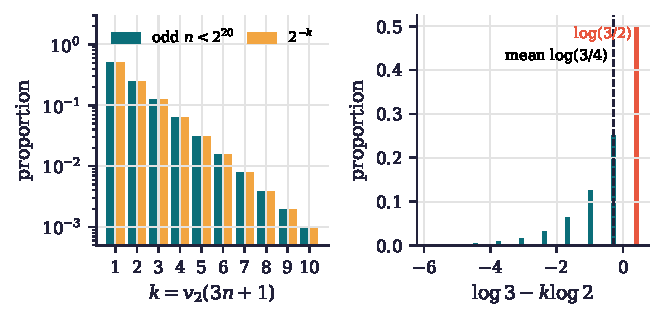
\includegraphics[width=\textwidth]{figures/ch2_syracuse.pdf}
\caption{Left: the proportion of odd $n<2^{20}$ with $\vt(3n+1)=k$ (dark bars) against the Geometric probabilities $2^{-k}$ (light bars); they agree exactly. Right: the induced law of $\log3-k\log2$, the multiplicative part of the Syracuse increment, with the single ascending value $\log(3/2)$, the only bar right of zero, and the mean $\log(3/4)$ dashed.}
\label{fig:ch2:syracuse}
\end{figure}

\begin{remark}[What the Geometric law does not say]\label{rem:ch2:notorbit}
\Cref{prop:geom} describes one Syracuse step from a random odd residue. Along
a single orbit the successive exponents $k_1,k_2,\ldots$ are deterministic.
Along an orbit that reaches $1$ they are eventually all equal to $2$, since $S(1)=1$; along a cycle with $r$ odd values and $s$ halvings in a period their running averages tend to $s/r$, which lies strictly between $\lt$ and $2$ unless the cycle is that of $1$ (summing \eqref{eq:ch2:stride} around the cycle gives $s\log2=\sum\log(3+1/y)$, a sum of $r$ terms in $(\log3,\log4]$, with $\log4$ only at $y=1$); and along a divergent orbit their upper limit is at most $\lt$ (\cref{cor:ch9:freq}).
So whether the running averages tend to $2$ along every orbit is the whole conjecture, and whether their lower limit exceeds $\lt$ along every orbit is exactly the divergence half (\cref{conj:cesaro}).
Taking logarithms in the
Syracuse orbit $x_t=S^{(t)}(n)$,
\[
  \log x_t=\log n+t\log3-(k_1+\cdots+k_t)\log2+\sum_{s<t}\log\Bigl(1+\frac1{3x_s}\Bigr),
\]
so an orbit along which $(k_1+\cdots+k_t)/t$ stays above $\lt+\varepsilon$ for
all large $t$ is bounded. \Cref{chap:divergence} studies this criterion and
its limitations.
\end{remark}

\section{The $2$ adic extension and the shift}\label{sec:ch2:adic}

\Cref{thm:terras} is a statement about every power of $2$ at once, and the
natural setting for such statements is the ring $\Ztwo$ of $2$ adic integers.
We recall what we need. Every $x\in\Ztwo$ has a unique expansion
$x=\sum_{i\geq0}x_i2^i$ with $x_i\in\{0,1\}$; the integers sit inside $\Ztwo$
(negative integers\index{negative cycles} having expansions with infinitely many ones, for instance
$-1=\sum_{i\geq0}2^i$), and so does every rational number with odd
denominator. The $2$ adic absolute value is $|x|_2=2^{-\vt(x)}$, and the balls
$a+2^k\Ztwo$ are both open and closed. Odd integers, and in particular $3$,
are units of $\Ztwo$. The Haar probability measure $\mu$ on $\Ztwo$ is the
unique Borel probability measure invariant under translation; it gives every
ball $a+2^k\Ztwo$ mass $2^{-k}$, and under $\mu$ the digits $x_0,x_1,\ldots$
are independent fair bits.

The accelerated map\index{accelerated map} extends to $\Ztwo$ by the same formula,
\[
  T(x)=\begin{cases}x/2,& x\in2\Ztwo,\\ (3x+1)/2,& x\notin2\Ztwo,\end{cases}
\]
and \cref{lem:ch2:perturb} holds verbatim for $x,a\in\Ztwo$, with the same
proof. Let $\Sigma=\{0,1\}^{\{0,1,2,\ldots\}}$ be the space of infinite binary
sequences with the shift $\mathrm{sh}(w_0,w_1,\ldots)=(w_1,w_2,\ldots)$, the metric
$d(w,w')=2^{-\min\{i:w_i\neq w'_i\}}$, and the Bernoulli product measure
$\beta$ under which the coordinates are independent fair bits. Define the
\emph{parity vector\index{parity vector} map}
\[
  Q:\Ztwo\to\Sigma,\qquad Q(x)=\bigl(T^{(i)}(x)\bmod2\bigr)_{i\geq0}.
\]

\begin{theorem}[Conjugacy to the shift]\label{thm:ch2:conj}
The map $Q$ has the following properties.
\begin{enumerate}[label=(\roman*),leftmargin=2em]
\item $Q$ is a bijective isometry from $(\Ztwo,|\cdot|_2)$ onto $(\Sigma,d)$.
\item $Q\circ T=\mathrm{sh}\circ Q$.
\item $Q$ carries the Haar measure $\mu$ to the Bernoulli measure $\beta$.
\item If $w\in\Sigma$ has ones at positions $d_1<d_2<\cdots$ (finitely or
  infinitely many), then
  \[
    Q^{-1}(w)=-\sum_{j\geq1}3^{-j}2^{d_j},
  \]
  the series converging in $\Ztwo$.
\end{enumerate}
\end{theorem}

The conjugacy (i) to (iii) was first stated explicitly by Lagarias\index{Lagarias, J. C.}~\cite[Theorem~L]{lagarias1985}, who records that it had been observed by Terras\index{Terras, R.} and Pomerance\index{Pomerance, C.}; it rests on the bijection of Terras~\cite{terras1976} and Everett\index{Everett, C. J.}~\cite{everett1977}.
The explicit inverse (iv) is due to
Bernstein\index{Bernstein, D. J.}~\cite{bernstein1994}. Since each part follows in a few lines from
what we have proved, we include the proofs.

\begin{proof}
(i) Let $x\neq y$ in $\Ztwo$ with $|x-y|_2=2^{-j}$, so $y=x+2^ja$ with $a$ a
unit. By \cref{lem:ch2:perturb}, $T^{(i)}(x)$ and $T^{(i)}(y)$ have the same
parity for $i<j$, while $T^{(j)}(y)-T^{(j)}(x)=3^{m_j(x)}a$ is a unit, so the
parities differ at $i=j$. Hence $d(Q(x),Q(y))=2^{-j}=|x-y|_2$. An isometry is
injective and continuous. For surjectivity, let $w\in\Sigma$. By
\cref{thm:terras} there is for each $k$ a unique residue $r_k\bmod2^k$ with
$v_k(r_k)=(w_0,\ldots,w_{k-1})$; since $v_k$ of a residue modulo $2^{k+1}$ is
the truncation of its $v_{k+1}$, we have $r_{k+1}\equiv r_k\pmod{2^k}$. The
compatible residues define $x\in\Ztwo$ with $x\equiv r_k\pmod{2^k}$ for all
$k$, and then the first $k$ entries of $Q(x)$ are $v_k(r_k)$, so $Q(x)=w$.

(ii) The $i$th entry of $Q(T(x))$ is the parity of $T^{(i+1)}(x)$, which is the
$(i+1)$st entry of $Q(x)$.

(iii) By (i), $Q$ maps each ball $x+2^k\Ztwo$ onto the cylinder of sequences
beginning with $v_k(x)$. Both have mass $2^{-k}$, under $\mu$ and $\beta$
respectively. Cylinders form a $\pi$ system generating the Borel
$\sigma$ algebra of $\Sigma$, so the probability measures $\beta$ and
$\mu\circ Q^{-1}$, which agree on cylinders, are equal.

(iv) Let $x=Q^{-1}(w)$. Reducing \eqref{eq:ch2:affine} modulo $2^k$ in $\Ztwo$
gives, as in \cref{cor:ch2:inverse},
$x\equiv-\sum_{j\leq m_k(x)}3^{-j}2^{d_j}\pmod{2^k}$. If $w$ has infinitely
many ones the terms satisfy $|3^{-j}2^{d_j}|_2=2^{-d_j}\to0$, so the series
converges; if finitely many, it is a finite sum. Letting $k\to\infty$ gives the
formula.
\end{proof}

\begin{figure}[ht]
\centering
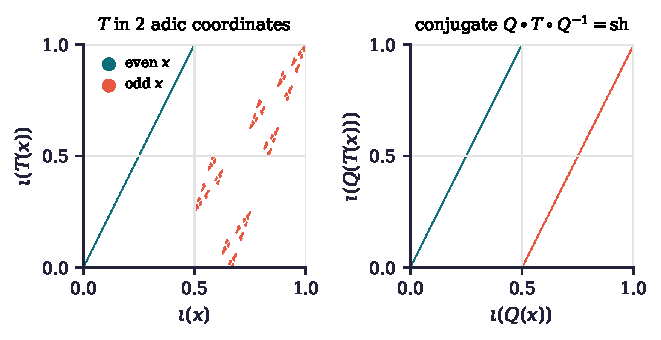
\includegraphics[width=\textwidth]{figures/ch2_adic_shift.pdf}
\caption{The conjugacy of \cref{thm:ch2:conj}, drawn on the residues modulo $2^{16}$. Left: the graph of $T$ in $2$ adic coordinates, a point $x=\sum x_i2^i$ being placed at $\iota(x)=\sum x_i2^{-i-1}\in[0,1)$; even points lie on one line of slope $2$ and odd points scatter. Right: in the coordinates given by the parity vector $Q$, the same map becomes the doubling map, the shift, with even and odd points on its two branches.}
\label{fig:ch2:adicshift}
\end{figure}

For example, $Q(0)=000\cdots$, and $Q(-1)=111\cdots$ since $T(-1)=-1$; indeed $-\sum_{j\geq1}3^{-j}2^{j-1}=-1$ in $\Ztwo$. Similarly $Q(1)=1010\cdots$, since $1\mapsto2\mapsto1$, and
$-\sum_{j\geq1}3^{-j}4^{j-1}=-\tfrac13(1-\tfrac43)^{-1}=1$, the geometric
series converging $2$ adically because $|4/3|_2=1/4$.

Part (iii) contains a measure preservation statement that we isolate, with a
direct proof that does not use the conjugacy.

\begin{proposition}[Haar measure is invariant]\label{prop:ch2:haar}
For every Borel set $A\subseteq\Ztwo$, $\mu(T^{-1}(A))=\mu(A)$.
\end{proposition}

\begin{proof}
It suffices to check balls $A=a+2^k\Ztwo$, since they form a $\pi$ system
generating the Borel sets. A point $x$ lies in $T^{-1}(A)$ either because $x$
is even and $x/2\in A$, that is $x\in2a+2^{k+1}\Ztwo$, or because $x$ is odd
and $(3x+1)/2\in A$, that is
\[
  x\in3^{-1}(2a-1)+2^{k+1}\Ztwo ,
\]
where we used that $3$ is a unit; the centre $3^{-1}(2a-1)$ is odd, so this
ball consists of odd points. The two balls are disjoint and each has measure
$2^{-k-1}$, so $\mu(T^{-1}(A))=2^{-k}=\mu(A)$.
\end{proof}

Since the Bernoulli shift is mixing\index{mixing}, \cref{thm:ch2:conj} shows that $T$ is a
mixing, in particular ergodic, transformation of $(\Ztwo,\mu)$ (Lagarias~\cite[Theorem~K]{lagarias1985}, as a special case of a result of Matthews\index{Matthews, K. R.} and Watts\index{Watts, A. M.}~\cite{matthews1984}).
This is the
cleanest statement of the randomness of the Collatz map, and it is
simultaneously the cleanest statement of why randomness does not suffice: the
positive integers form a set of Haar measure\index{Haar measure} zero in $\Ztwo$, and ergodic
theory is silent about null sets. Inside $\Ztwo$ the conjecture takes the
following form.

\begin{corollary}\label{cor:ch2:tail}
An integer $n\geq1$ satisfies $T^{(k)}(n)=1$ if and only if $\mathrm{sh}^kQ(n)=1010\cdots$.
Hence the Collatz conjecture\index{Collatz conjecture} is equivalent to the statement that the parity
vector of every positive integer ends in the periodic tail $1010\cdots$.
\end{corollary}

\begin{proof}
By (ii), $\mathrm{sh}^kQ(n)=Q(T^{(k)}(n))$, and by (i) this equals $Q(1)$ if and
only if $T^{(k)}(n)=1$.
\end{proof}

\begin{remark}[Rational points and periodic sequences]\label{rem:ch2:periodic}
If $w$ is eventually periodic, then the series in (iv) is eventually a
geometric series and $Q^{-1}(w)$ is a rational number with odd denominator.
The converse, that $Q$ maps every rational number with odd denominator to an
eventually periodic sequence, is the \emph{periodicity conjecture} of
Lagarias~\cite{lagarias1985,lagarias1990}. It would imply that no orbit of a
positive integer is unbounded: if $Q(n)$ is eventually periodic, say
$\mathrm{sh}^{k+p}Q(n)=\mathrm{sh}^kQ(n)$, then $T^{(k+p)}(n)=T^{(k)}(n)$ by
injectivity of $Q$, and the orbit is eventually periodic.
\end{remark}

\section{Stopping times and the density theorem}\label{sec:ch2:density}

\begin{definition}[Stopping times]\label{def:ch2:stopping}
For $n\geq1$ the \emph{stopping time\index{stopping time}} is
$\sigma(n)=\min\{k\geq1:T^{(k)}(n)<n\}$, with $\sigma(n)=\infty$ if there is no
such $k$. The \emph{coefficient stopping time\index{coefficient stopping time}} is
\[
  \tau(n)=\min\{k\geq1:3^{m_k(n)}<2^k\},
\]
the first time the multiplicative coefficient in \eqref{eq:ch2:affine} drops
below $1$.
\end{definition}

If every $n\geq2$ has finite stopping time then the conjecture follows by
strong induction, since the orbit of $n$ reaches a smaller value whose orbit
reaches $1$. Conversely, under the conjecture every $n\geq2$ has finite
stopping time. Note that $\sigma(1)=\infty$ trivially, because the orbit of $1$
never goes below $1$. The coefficient stopping time is a function of the
parity vector\index{parity vector} alone, and therefore of a residue class: if $\tau(n)=k$ then
$\tau(n')=k$ for every $n'\equiv n\pmod{2^k}$.

The following facts, and the exact counts of \cref{sec:ch2:dp}, are due to Terras\index{Terras, R.}~\cite{terras1976} (his Proposition~1.8 and Theorems~1.9, 1.14 and~2.1); see also \cite[Theorem~C]{lagarias1985}.

\begin{proposition}[Stopping times and coefficient stopping times]\label{prop:ch2:tau}
\leavevmode
\begin{enumerate}[label=(\roman*),leftmargin=2em]
\item $\tau(n)\leq\sigma(n)$ for every $n\geq1$.
\item If $\tau(n)=k$ and $m=m_k(n)$, then $\sigma(n')=k$ for every
  $n'\equiv n\pmod{2^k}$ with $n'>c_k(n)/(2^k-3^m)$.
\item If $\tau(n)<\infty$, then $\tau(n)=\lfloor m\lt\rfloor+1$ with
  $m=m_{\tau(n)}(n)$, and the last entry of $v_{\tau(n)}(n)$ is $0$.
\end{enumerate}
\end{proposition}

\begin{proof}
(i) If $T^{(k)}(n)<n$ then by \eqref{eq:ch2:affine}
$3^{m_k}n+c_k=2^kT^{(k)}(n)<2^kn$, and since $c_k\geq0$ this forces
$3^{m_k}<2^k$. So $\tau(n)\leq k$ for every such $k$.

(ii) For $n'$ in the class, $\tau(n')=k$ and $c_k(n')=c_k(n)$, so
$T^{(k)}(n')<n'$ if and only if $3^mn'+c_k(n)<2^kn'$, which is the stated
condition. Then $\sigma(n')\leq k$, and $\sigma(n')\geq\tau(n')=k$ by (i).

(iii) Let $k=\tau(n)<\infty$ and $m=m_k(n)$. If $k=1$ then $n$ is even, $m=0$ and
$k=\lfloor0\rfloor+1$. If $k\geq2$ then $3^{m_{k-1}}\geq2^{k-1}$, and in fact
$3^{m_{k-1}}>2^{k-1}$ since a power of $3$ equals a power of $2$ only when
both are $1$. If the last step were odd we would have $m=m_{k-1}+1$ and
$3^m>3\cdot2^{k-1}>2^k$, contradicting $3^m<2^k$. So the last step is even,
$m=m_{k-1}$, and $2^{k-1}<3^m<2^k$, which says $k-1<m\lt<k$, that is
$k=\lfloor m\lt\rfloor+1$.
\end{proof}

By (iii), finite coefficient stopping times can take only the values $1$, $2$, $4$, $5$, $7$,
$8$, $10$, $12$, $13$, $15$, $16$, $18$, $20$, and so on; the gaps at $3$,
$6$, $9$, $11$, $14$, $17$, $19$, and so on, are the integers
not of the form $\lfloor m\lt\rfloor+1$. By (ii) the same restriction applies
to $\sigma(n)$ for all sufficiently large $n$ in each class with finite $\tau$,
and \cref{prop:ch2:dp} below shows that every value in the list is actually
taken by some residue class.

\begin{example}\label{ex:ch2:stop}
Even $n$ have $\sigma(n)=1$. If $n\equiv1\pmod4$ then the parity vector of length $2$ is $(1,0)$, so
$\tau(n)=2$, $c_2=1$, and $T^{(2)}(n)=(3n+1)/4<n$ for all $n>1$. If
$n\equiv3\pmod{16}$ then $v_4(n)=(1,1,0,0)$, so $m=2$, $c_4=3+2=5$,
$2^4-3^2=7$, and $T^{(4)}(n)=(9n+5)/16<n$ for every $n\geq1$ in the class. In
the other classes modulo $16$, namely $7,11,15\pmod{16}$, the first four
steps do not yet decide.
\end{example}

\Cref{fig:ch2:stopheat} shows the same phenomenon on actual integers. The
stopping times $\sigma(n)$ of $2\leq n<2^{13}$ are arranged in rows of $64$,
so that each column is a residue class modulo $64$. In $56$ of the $64$
columns the stopping time is constant: it is the coefficient stopping time
of the class, reached within six steps. The remaining eight columns are the
classes modulo $64$ whose first six parities do not yet decide, and only there
does the stopping time vary from row to row.

\begin{figure}[t]
\centering
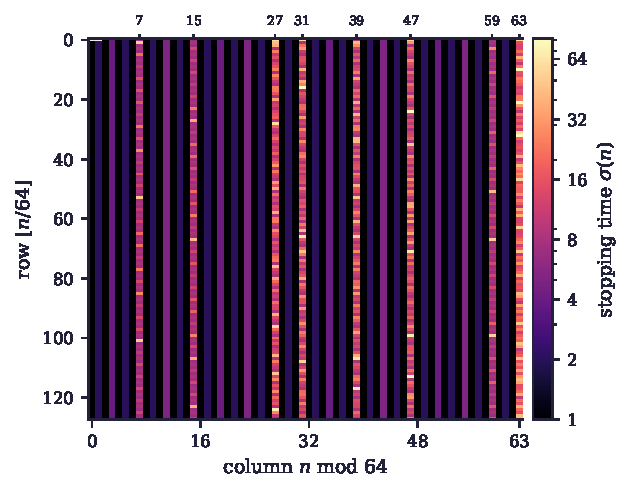
\includegraphics[width=\textwidth]{figures/ch2_stopheat.pdf}
\caption{Stopping times $\sigma(n)$ for $2\leq n<2^{13}$, arranged with $n$ in
row $\lfloor n/64\rfloor$ and column $n\bmod64$, on a logarithmic colour
scale ($n=0,1$ are left blank). Fifty six columns are constant, because
$\tau\leq6$ on them and $\sigma=\tau$ there; the eight columns $7$, $15$,
$27$, $31$, $39$, $47$, $59$, $63$ marked at the top are the classes with
$\tau>6$, a proportion $1/8$ of all classes.}
\label{fig:ch2:stopheat}
\end{figure}

\subsection{Exact counts}\label{sec:ch2:dp}

The number of residue classes that stop at each step can be computed exactly,
without enumerating residues, by a dynamic programme over the number of odd
steps. Call a word $w\in\{0,1\}^k$ \emph{alive} if $3^{m_j(w)}>2^j$ for
$1\leq j\leq k$, where $m_j(w)$ is the number of ones among its first $j$
letters; by \cref{thm:terras} the alive words of length $k$ are the parity
vectors of the residue classes modulo $2^k$ with $\tau>k$. (Since a power of
$3$ never equals a positive power of $2$, the alternative to alive is
$3^{m_j}<2^j$ for some $j$.) Write
\begin{gather*}
  N_k(m)=\#\{w\in\{0,1\}^k\text{ alive}:m_k(w)=m\},\\
  R_k=\#\{r\bmod2^k:\tau(r)=k\}.
\end{gather*}

\begin{proposition}[Exact stopping counts]\label{prop:ch2:dp}
\leavevmode
\begin{enumerate}[label=(\roman*),leftmargin=2em]
\item $N_0(0)=1$, and for $k\geq1$ and $m\geq0$,
  \[
    N_k(m)=\bigl(N_{k-1}(m)+N_{k-1}(m-1)\bigr)\,[\,3^m>2^k\,],
  \]
  with $N_{k-1}(-1)=0$, where $[P]$ is $1$ if $P$ holds and $0$ otherwise. The
  proportion of residues modulo $2^k$ with $\tau>k$
  is $1-F(k)=2^{-k}\sum_mN_k(m)$, and among them the number of odd steps
  in the first $k$ has the law $m\mapsto N_k(m)/\sum_{m'}N_k(m')$.
\item There is at most one integer $m^\ast_k\geq0$ with $2^{k-1}\leq3^{m^\ast_k}<2^k$; equality on the left occurs only for $k=1$ and $m^\ast_1=0$.
  If it exists then $R_k=N_{k-1}(m^\ast_k)\geq1$, and otherwise $R_k=0$.
  Consequently $R_k>0$ if and only if $k=\lfloor m\lt\rfloor+1$ for some
  integer $m\geq0$.
\item The counts satisfy $2^k\bigl(1-F(k)\bigr)=2^{k}\bigl(1-F(k-1)\bigr)-R_k$
  and $F(k)=\sum_{j\leq k}R_j2^{-j}$.
\end{enumerate}
\end{proposition}

\begin{proof}
(i) A word of length $k$ is alive exactly when its prefix of length $k-1$ is
alive and $3^{m_k}>2^k$. Splitting according to the last letter, which is $0$
or $1$, gives the recursion. The statements about residues follow from
\cref{thm:terras}, which makes the parity vector\index{parity vector} of a uniform residue modulo
$2^k$ uniform on $\{0,1\}^k$.

(ii) The condition $2^{k-1}\leq3^m<2^k$ says that $m$ lies in the half open
interval $\bigl[(k-1)/\lt,\,k/\lt\bigr)$, of length $1/\lt<1$, so it has at
most one solution. A residue has $\tau=k$ exactly when its parity word of
length $k$ has an alive prefix of length $k-1$ and $3^{m_k}<2^k$. By
\cref{prop:ch2:tau}(iii) its last letter is then $0$ and $m=m_{k-1}=m_k$
satisfies $2^{k-1}\leq3^m<2^k$ (for $k=1$ the word is $0$ and $m=0$), so $m=m^\ast_k$. Conversely, every alive word of
length $k-1$ with $m^\ast_k$ ones, followed by a $0$, has $\tau=k$. Hence
$R_k=N_{k-1}(m^\ast_k)$. The word $1^{m}0^{k-1-m}$ with $m=m^\ast_k$ is alive,
since $3^{j}>2^{j}$ for $1\leq j\leq m$ and $3^m>2^{j}$ for $m<j\leq k-1$, so $R_k\geq1$. Finally
$m^\ast_k$ exists if and only if $k-1\leq m\lt<k$ for some integer $m\geq0$, that is,
$k=\lfloor m\lt\rfloor+1$.

(iii) Each alive word of length $k-1$ has two extensions, and exactly the
$R_k$ extensions counted in (ii) fail to be alive. The second identity
follows by summing.
\end{proof}

\Cref{tab:ch2:residues} lists $R_k$ and $1-F(k)$ for $k\leq40$, computed
from the recursion with exact integer arithmetic, and \cref{fig:ch2:tree}
draws the first seven levels as a tree. For small $k$ the classes are easily
listed: $\tau=1$ on $0\bmod2$, $\tau=2$ on $1\bmod4$, $\tau=4$ on $3\bmod16$,
$\tau=5$ on $11$ and $23\bmod32$, $\tau=7$ on $7$, $15$ and $59\bmod128$, and
$\tau=8$ on $39$, $79$, $95$, $123$, $175$, $199$ and $219\bmod256$. The
recursion has been checked against direct enumeration of all residues for
$k\leq20$, and the equivalence in (ii) against the recursion for $k\leq400$
(script \texttt{ch02\_exact.py}). \Cref{fig:ch2:sunburst} displays the whole
alive tree to depth nine, coloured by the height $m_k\log3-k\log2$, the
logarithm of the coefficient $3^{m_k}/2^k$ in \eqref{eq:ch2:affine}; a class
stops at the first ring where its height becomes negative.

\begin{table}[t]
\centering
\caption{Number $R_k$ of residue classes modulo $2^k$ with coefficient
stopping time $\tau=k$, and the proportion $1-F(k)$ of residues modulo $2^k$
with $\tau>k$, from \cref{prop:ch2:dp}. The rows with $R_k=0$ are the $k$
not of the form $\lfloor m\lt\rfloor+1$.
Terras~\cite{terras1976} tabulates the same distribution to $k=900$ (his Table~A).}
\label{tab:ch2:residues}
\small\setlength{\tabcolsep}{5pt}
\begin{tabular}{@{}rrr@{\hspace{14pt}}rrr@{}}
\toprule
$k$ & $R_k$ & $1-F(k)$ & $k$ & $R_k$ & $1-F(k)$\\
\midrule
$1$ & $1$ & $0.500000$ & $21$ & $8045$ & $0.022226$\\
$2$ & $1$ & $0.250000$ & $22$ & $0$ & $0.022226$\\
$3$ & $0$ & $0.250000$ & $23$ & $17\,637$ & $0.020123$\\
$4$ & $1$ & $0.187500$ & $24$ & $51\,033$ & $0.017082$\\
$5$ & $2$ & $0.125000$ & $25$ & $0$ & $0.017082$\\
$6$ & $0$ & $0.125000$ & $26$ & $108\,950$ & $0.015458$\\
$7$ & $3$ & $0.101562$ & $27$ & $312\,455$ & $0.013130$\\
$8$ & $7$ & $0.074219$ & $28$ & $0$ & $0.013130$\\
$9$ & $0$ & $0.074219$ & $29$ & $663\,535$ & $0.011894$\\
$10$ & $12$ & $0.062500$ & $30$ & $0$ & $0.011894$\\
$11$ & $0$ & $0.062500$ & $31$ & $1\,900\,470$ & $0.011009$\\
$12$ & $30$ & $0.055176$ & $32$ & $5\,936\,673$ & $0.009627$\\
$13$ & $85$ & $0.044800$ & $33$ & $0$ & $0.009627$\\
$14$ & $0$ & $0.044800$ & $34$ & $13\,472\,296$ & $0.008843$\\
$15$ & $173$ & $0.039520$ & $35$ & $39\,993\,895$ & $0.007679$\\
$16$ & $476$ & $0.032257$ & $36$ & $0$ & $0.007679$\\
$17$ & $0$ & $0.032257$ & $37$ & $87\,986\,917$ & $0.007039$\\
$18$ & $961$ & $0.028591$ & $38$ & $0$ & $0.007039$\\
$19$ & $0$ & $0.028591$ & $39$ & $257\,978\,502$ & $0.006569$\\
$20$ & $2652$ & $0.026062$ & $40$ & $820\,236\,724$ & $0.005823$\\
\bottomrule
\end{tabular}
\end{table}

\begin{figure}[tp]
\centering
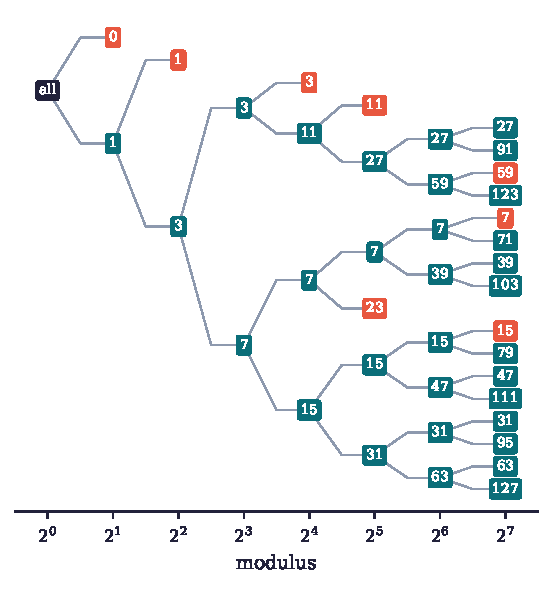
\includegraphics[width=\textwidth]{figures/ch2_residue_tree.pdf}
\caption{The stopping tree. A node at modulus $2^j$ is a residue class modulo $2^j$ whose orbit has not stopped before step $j$. Lighter nodes stop at step $j$ ($\tau=j$) and are leaves; each darker node $r$ splits into the classes $r$ and $r+2^j$ modulo $2^{j+1}$. At modulus $2^7$, $13$ of the $128$ classes remain.}
\label{fig:ch2:tree}
\end{figure}

\begin{figure}[tp]
\centering
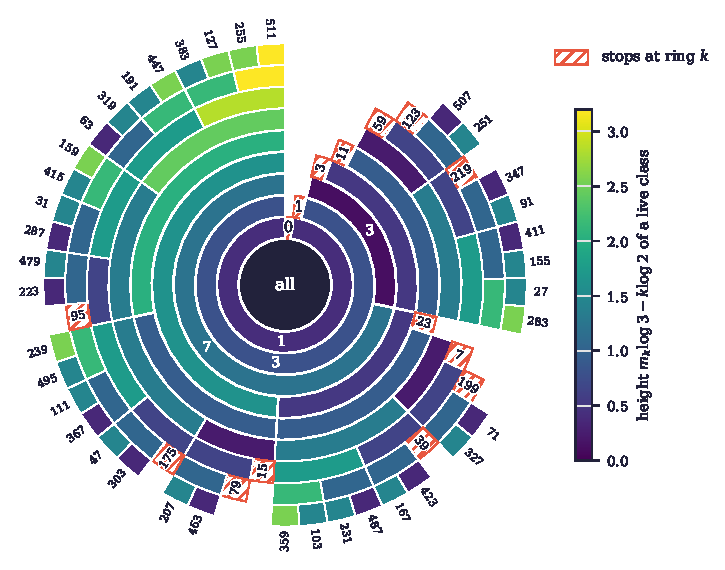
\includegraphics[width=\textwidth]{figures/ch2_sunburst.pdf}
\caption{The Terras parity tree as a sunburst. Ring $k$ consists of residue classes modulo $2^k$, equivalently parity words of length $k$, and the two children of a class in ring $k+1$ are its two lifts. A class that stops at ring $k$ ($\tau=k$) is a hatched wedge labelled by its residue with nothing outside it; live classes are shaded by their height $m_k\log3-k\log2$. Angular width is proportional to the number of leaves below a node, not to Haar measure. The outer labels are the $38$ classes modulo $2^9$ with $\tau>9$.}
\label{fig:ch2:sunburst}
\end{figure}

We can now prove the theorem of Terras\index{Terras, R.} and Everett\index{Everett, C. J.}, in the quantitative form given by Lagarias\index{Lagarias, J. C.}~\cite[Theorem~D]{lagarias1985}.
Write
\[
  F(k)=2^{-k}\,\#\{r\bmod2^k:\tau(r)\leq k\},\qquad
  \theta=\frac{\log2}{\log3}\approx0.6309,
\]
and let
\[
  D=\theta\log(2\theta)+(1-\theta)\log\bigl(2(1-\theta)\bigr)\approx0.03469
\]
be the Kullback\index{Kullback and Leibler divergence} and Leibler divergence of the Bernoulli$(\theta)$ law from the
Bernoulli$(\tfrac12)$ law.
(In this section only, $\theta$ denotes $1/\lt$, the threshold frequency of odd steps; in \cref{chap:cycles} it denotes $\lt$ itself.)

\begin{theorem}[{Terras~\cite{terras1976,terras1979}, Everett~\cite{everett1977}, Lagarias~\cite[Theorem~D]{lagarias1985}}]\label{thm:density}
For each $k\geq1$ the set $\{n\geq1:\sigma(n)\leq k\}$ has natural density
$F(k)$, and
\[
  1-F(k)\leq e^{-Dk}.
\]
Consequently the set of $n\geq1$ with finite stopping time\index{stopping time} has natural
density $1$.
\end{theorem}

\begin{proof}
\emph{Step 1: the coefficient stopping time\index{coefficient stopping time}.} The set $A_k=\{n\geq1:
\tau(n)\leq k\}$ is a union of residue classes modulo $2^k$: whether
$\tau(n)\leq k$ is decided by $v_k(n)$, hence by $n\bmod2^k$. A union of $R$
classes modulo $2^k$ has natural density $R/2^k$, so $A_k$ has density $F(k)$.

\emph{Step 2: comparison with the stopping time.} Let $B_k=\{n\geq1:
\sigma(n)\leq k\}$. By \cref{prop:ch2:tau}(i), $B_k\subseteq A_k$. Conversely,
each class $r\bmod2^j$ with $\tau=j\leq k$ is contained in $B_k$ apart from the
finitely many $n\leq c_j(r)/(2^j-3^{m_j(r)})$, by \cref{prop:ch2:tau}(ii). There
are finitely many such classes, so $A_k\setminus B_k$ is finite, and $B_k$ has
the same density $F(k)$ as $A_k$.

\emph{Step 3: reduction to a binomial tail.} By \cref{cor:ch2:iid}, $1-F(k)$
is the probability that a uniformly random word $w\in\{0,1\}^k$ satisfies
$3^{m_j(w)}\geq2^j$ for every $j\leq k$, where $m_j(w)$ is the number of ones
among the first $j$ letters. In particular such a word has $3^{m_k(w)}\geq2^k$,
that is $m_k(w)\geq\theta k$. Hence
\[
  1-F(k)\leq\Prob(X\geq\theta k),\qquad X\sim\mathrm{Binomial}(k,\tfrac12).
\]

\emph{Step 4: the Chernoff\index{large deviations} bound.} For every $\lambda>0$, Markov's inequality
applied to $e^{\lambda X}$ gives
\[
  \Prob(X\geq\theta k)\leq e^{-\lambda\theta k}\,\E e^{\lambda X}
  =\Bigl(e^{-\lambda\theta}\,\frac{1+e^{\lambda}}{2}\Bigr)^{k}.
\]
Since $\theta>\tfrac12$ we may take $e^{\lambda}=\theta/(1-\theta)>1$. Then
$(1+e^\lambda)/2=1/(2(1-\theta))$ and $e^{-\lambda\theta}=((1-\theta)/\theta)^{\theta}$,
and the logarithm of the bracket is
\begin{align*}
  -\theta\log\frac{\theta}{1-\theta}&-\log\bigl(2(1-\theta)\bigr)\\
  &=-\theta\log(2\theta)-(1-\theta)\log\bigl(2(1-\theta)\bigr)=-D .
\end{align*}
So $1-F(k)\leq e^{-Dk}$.

\emph{Step 5: conclusion.} The set $B=\{n:\sigma(n)<\infty\}$ contains $B_k$
for every $k$, so its lower density is at least $F(k)\geq1-e^{-Dk}$ for every
$k$. Since $D>0$, the lower density of $B$ is $1$, and hence $B$ has natural
density $1$.
\end{proof}

\begin{figure}[tp]
\centering
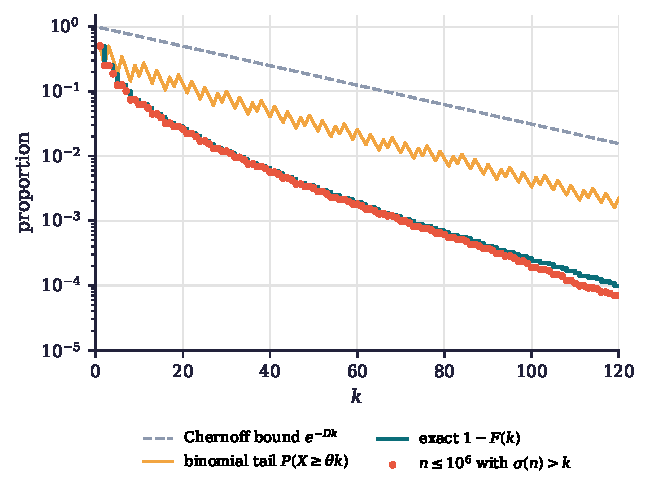
\includegraphics[width=\textwidth]{figures/ch2_stopdecay.pdf}
\caption{Decay of the proportion of residues that have not stopped. Dark solid line: the exact density $1-F(k)$ of $\{\tau>k\}$. Dots: the fraction of $n\leq10^6$ with $\sigma(n)>k$. Light solid line: the binomial tail used in Step 3 of the proof. Dashed line: the Chernoff bound $e^{-Dk}$.}
\label{fig:ch2:stopdecay}
\end{figure}

\Cref{fig:ch2:stopdecay} compares the exact proportion $1-F(k)$, computed by
dynamic programming over the number of ones in the parity word, with the
bounds used in the proof. The bound is valid but loose: at $k=100$ the exact
value is $2.39\times10^{-4}$, the binomial tail is $3.32\times10^{-3}$, and the
Chernoff bound is $3.12\times10^{-2}$. The ratio $(1-F(k))/e^{-Dk}$ falls
from $0.052$ at $k=20$ to $0.0077$ at $k=100$ and $0.0032$ at $k=200$. Step 3
throws away the requirement that the walk $j\mapsto m_j\log3-j\log2$ stay
nonnegative at every intermediate time and keeps only the endpoint.
This loses at most a factor $k$ (\cref{ex:ch2:sharp}), so the exponent $D$ cannot be improved, as Lagarias\index{Lagarias, J. C.}~\cite{lagarias1985} observes.
The endpoint probability is of order $k^{-1/2}e^{-Dk}$, and for a random walk with negative drift\index{drift} the probability of staying above a barrier for $k$ steps is, heuristically, smaller by a further factor of order $k^{-1}$, so of order $k^{-3/2}e^{-Dk}$.
The local exponent of the observed ratio to $e^{-Dk}$, $-1.19$ between $k=20$ and $k=100$ and $-1.41$ between $k=400$ and $k=800$, approaches $-3/2$ slowly; we do not need or prove this refinement.

Two further remarks place the theorem in context.

\begin{remark}[The coefficient stopping time conjecture]\label{rem:ch2:cst}
We always have $\tau\leq\sigma$ by \cref{prop:ch2:tau}, with equality
for all sufficiently large members of each class.
Terras~\cite{terras1976} conjectured that every $n\geq2$ has $\sigma(n)=\tau(n)$, verified this for $n<250\,000$, and deduced from an explicit bound that it holds for every $n$ with $\tau(n)<2592$; see Lagarias\index{Lagarias, J. C.}~\cite[Theorem~H]{lagarias1985}.
We have also checked it directly for $2\leq n\leq10^6$.
The
conjecture would rule out nontrivial cycles: if $n\geq2$ were the least
element of a cycle of length $k$ with $m$ odd elements, then $\sigma(n)=\infty$,
while $3^m<2^k$ by \cref{cor:ch2:cycle}, so $\tau(n)\leq k$. It says nothing
directly about unbounded orbits, since a starting value of such an orbit
could have $\tau=\infty$ as well. Among
$n\leq10^6$ the largest stopping time is $\sigma(626\,331)=176$; half of all
$n$ have $\sigma(n)=1$ and a quarter have $\sigma(n)=2$, in agreement with
\cref{tab:ch2:residues}.
\end{remark}

\begin{remark}[Why density one is not enough]\label{rem:ch2:notenough}
\Cref{thm:density} says that almost every $n$ falls below itself. It does not
say that almost every $n$ reaches $1$. To descend from $n$ to $1$ an orbit
must pass through a chain of smaller values each of which must itself have
finite stopping time, and the exceptional set, though of density zero, might
contain a value on every orbit. Repeating the argument from the value
$T^{(\sigma(n))}(n)$ is not legitimate, because that value is not uniformly
distributed in any residue class: it is determined by $n$, and its residues
have been used up in computing $\sigma(n)$. This is the gap between ensemble
and orbit that recurs throughout the book. Results that go further, from
Korec\index{Korec, I.}'s exponent $\log3/\log4$ to Tao\index{Tao, T.}'s almost bounded values, are described
in \cref{chap:intro}.
\end{remark}

\section*{Notes}

The parity vector\index{parity vector} and its bijection with residues are due to
Terras\index{Terras, R.}~\cite{terras1976} and Everett\index{Everett, C. J.}~\cite{everett1977}; see \cite[Theorem~B]{lagarias1985}.
Terras also introduced the coefficient stopping time\index{coefficient stopping time}\index{stopping time}, proved the facts collected in \cref{prop:ch2:tau}, gave the recursion of \cref{prop:ch2:dp} with a table of the resulting distribution (his Table~A) and the description of the values of $\tau$ with a table of them (his Table~B), proved that the limiting distribution $F(k)$ exists, as in Steps 1 and 2 of the proof of \cref{thm:density}, and, by the central limit theorem, that $F(k)\to1$, which is the density statement of \cref{thm:density} (further details of the proof are in a later note~\cite{terras1979}), and stated the coefficient stopping time conjecture.
The density
statement was proved independently by Everett~\cite{everett1977}, who worked
with $f(2n)=n$, $f(2n+1)=3n+2$, which is our accelerated map\index{accelerated map} $T$.
The exponential bound of \cref{thm:density} is Theorem~D of Lagarias\index{Lagarias, J. C.}~\cite{lagarias1985}, proved there by bounding the same binomial tail; Lagarias also observes that its exponent cannot be improved.
The survey of
Lagarias\index{Lagarias, J. C.}~\cite{lagarias1985} gives a unified account of these results, the
$2$ adic extension and the conjugacy of \cref{thm:ch2:conj}, and many
generalizations; its section on the $2$ adic viewpoint is still the best
introduction. Bernstein\index{Bernstein, D. J.}~\cite{bernstein1994} gave the noniterative formula
for $Q^{-1}$, and the rational cycles\index{rational cycles} of the extended map are studied by
Lagarias~\cite{lagarias1990}. Wirsching\index{Wirsching, G. J.}~\cite{wirsching1998} develops the
combinatorics of parity words and of the inverse tree\index{inverse tree} in depth.
The identity $T^{(j)}(2^ja-1)=3^ja-1$ of \cref{rem:ch2:pitfall} is classical; see
Hercher\index{Hercher, C.}~\cite[Lemma~8]{hercher2023}, who cites Terras~\cite{terras1976} for it.

The affine identity \eqref{eq:ch2:affine} and the cycle formula
\eqref{eq:ch2:cyclen} are classical and appear, in various notations, in most
treatments of cycles; we have followed the notation of our Lean\index{Lean} formalization,
in which the recursion \eqref{eq:ch2:crec} is the inductive step of the proof.
The sum \eqref{eq:ch2:cexplicit} is a sum of terms $3^j2^i$ indexed by the
parity word, and the question of whether its structure, rather than only its
size, can constrain cycles is one of the open problems of \cref{chap:open}.

The Chernoff\index{large deviations} argument in Step 4 is the simplest route to an explicit rate; the
true asymptotics of $1-F(k)$ are those of the probability that a random walk with negative drift\index{drift} stays positive for $k$ steps.
\Cref{chap:stochastic} recovers the same
exponential rate for the first descent of the stochastic model, though not the
finer asymptotics.

\section*{Exercises}

\begin{exercise}\label{ex:ch2:runs}
Prove the identity $T^{(i)}(2^ja-1)=3^i2^{j-i}a-1$ of \cref{rem:ch2:pitfall}.
Deduce that $T^{(j)}(2^j-1)=3^j-1$, and that for every $j$ there are infinitely
many $n$ whose orbits under $T$ begin with exactly $j$ odd steps followed by an
even step.
\end{exercise}

\begin{exercise}\label{ex:ch2:bernstein}
Use \cref{thm:ch2:conj}(iv) to find the $2$ adic integer whose parity vector\index{parity vector}
is the periodic word $110110\cdots$, and show that it is $-5$. Explain the answer in terms of the cycle
$-5\mapsto-7\mapsto-10\mapsto-5$. More generally, show that if $w$ is periodic
with period $k$ and has $m$ ones in each period, then $Q^{-1}(w)=c(w)/(2^k-3^m)$
with $c(w)$ the sum \eqref{eq:ch2:cexplicit} over one period, in agreement with
\cref{cor:ch2:cycle}.
\end{exercise}

\begin{exercise}\label{ex:ch2:class11}
For $n\equiv11\pmod{32}$ compute $v_5(n)$, $m_5(n)$ and $c_5(n)$, and show that
$T^{(5)}(n)=(27n+23)/32$. Deduce that $\sigma(n)=5$ for every such $n$, and
compute the natural densities of $\{\sigma=4\}$ and $\{\sigma=5\}$.
\end{exercise}

\begin{exercise}\label{ex:ch2:syrhaar}
Let $U=\Ztwo\setminus2\Ztwo$ be the $2$ adic units with normalized Haar measure\index{Haar measure}
$\mu_U=2\mu|_U$, and extend the Syracuse map\index{Syracuse map} to $U\setminus\{-1/3\}$. Show
that for an odd ball $b+2^k\Ztwo$ the preimage under $S$ is the disjoint union
over $j\geq1$ of the balls $3^{-1}(2^jb-1)+2^{k+j}\Ztwo$, and deduce that $S$
preserves $\mu_U$. Show that under $\mu_U$ the halving exponent of $S$ has
exactly the Geometric$(\tfrac12)$ law.
\end{exercise}

\begin{exercise}\label{ex:ch2:sharp}
Let $X$ and $\theta$ be as in the proof of \cref{thm:density}. Let $w\in\{0,1\}^k$ satisfy $3^{m_k(w)}>2^k$, and let $j$ be the last index in $\{0,\ldots,k-1\}$ at which $m_j(w)\log3-j\log2$ is smallest. Show that the word obtained from $w$ by moving its first $j$ letters to the end is alive, in the sense of \cref{sec:ch2:dp}, and deduce that $\Prob(X\geq\theta k)/k\leq1-F(k)\leq\Prob(X\geq\theta k)$. Using $\binom ki\geq2^{kH(i/k)}/(k+1)$, where $H(x)=-x\log_2x-(1-x)\log_2(1-x)$, and $D=(1-H(\theta))\log2$, show that $\frac1k\log\bigl(1-F(k)\bigr)\to-D$, so that the exponent in \cref{thm:density} cannot be improved.
\end{exercise}

\begin{exercise}\label{ex:ch2:standard}
Formulate and prove the analogue of \cref{thm:terras} for the standard map\index{standard map}
$T_0$. Show that the parity vectors of length $k$ under $T_0$ are exactly the
binary words with no two consecutive ones, that their number is the
Fibonacci number $\mathrm{Fib}_{k+2}$ (with $\mathrm{Fib}_1=\mathrm{Fib}_2=1$), and that the set of $n$ with a given word $w$ is a
single residue class modulo $2^{z+1}$, where $z$ is the number of zeros among
the first $k-1$ letters of $w$. Explain why there is no longer a bijection
with the residues modulo a fixed power of $2$.
\end{exercise}
